
\section{Vectores}

\subsection{vectores}

 un vector es un ente matematico, es decir, es una figura creada para dar
    forma a la realidad como lo son la recta o el plano. Fue creada para
    representar fenomenos que no pueden ser descritos solamente con numeros, por
    ejemplo, la velocidad y las fuerzas. Son, por tanto, una construccion
    mas compleja que  la de los numeros y representan \textbf{una magnitud con
    direccion y sentido}. Graficamente son representados como una recta con
    cierto angulo de inclinacion y un sentido marcado por ua flechita, la
    direccion a la que apuntan.  Para poder representar un vector se necesitan
    al menos 2 puntos, el inicio del vector y el final (graficamente, si unes 2
    puntos obtienes una recta, algebraicamente se restan $punto_{final}-
    punto_{inicial}=magnitud_{vector}$ )

    Existen muchos vectores,y estos son utilizados para dar representacion a
    fenomenos fisicos. En general un vector de dimension $n$ es una tupla (un
    conjunto ordenado invariable de la forma $(x_1,x_2,\cdots,x_n)$ de numeros
    reales.

    Un vector posee 2 caracteristicas:

    \begin{itemize} \item Modulo, es su valor, la longitud del segmento o la
                cantidad de espacios que se mueve en un determinado eje (o
                ejes).

        \item Direccion, En algunos textos se descompone como direccion y
            sentido.  Es el angulo del segmento con respecto a un eje
            (normalmente x) y su sentido con respecto al origen (va o no hacia
            ese punto). Ejemplo: $29^o$ noreste sentido hacia arriba.
    \end{itemize}

    Graficamente un vector de 2 dimensiones en el origen se ve de la forma:

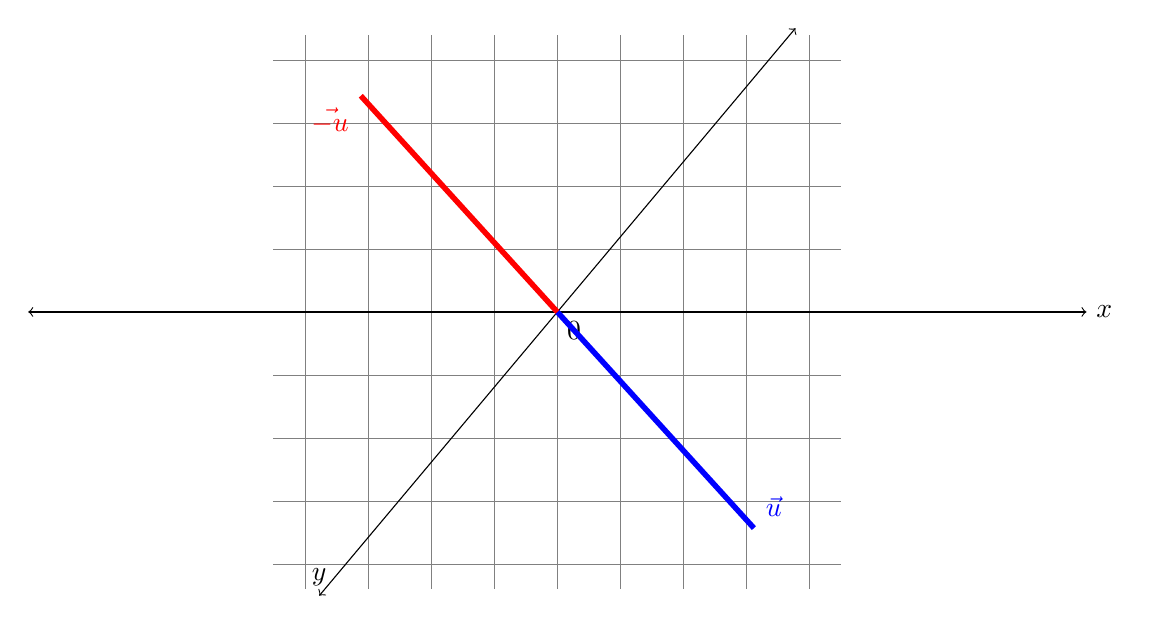
\begin{tikzpicture}[scale=1.6]

    \draw[style=help lines,step=0.5cm] (-4.1,-4.1)grid(4.1,4.1);

    \draw[<->] (-4.2,0)--(4.2,0) node[right]{$x$};
    \draw[<->] (0,-4.2)--(0,4.2) node[above]{$y$};
    \draw (0,0) node[anchor=north west ]{0};

    \draw[line width=2pt,blue](0,0)--(3,3.2) node[anchor=south west]{$\boldsymbol{\vec{u}}$};
    \draw[line width=2pt,red](0,0)--(-3,-3.2) node[anchor=north east]{$\boldsymbol{\vec{-u}}$};
\end{tikzpicture}

y de 3 dimensiones, en el origen se ve de la forma:


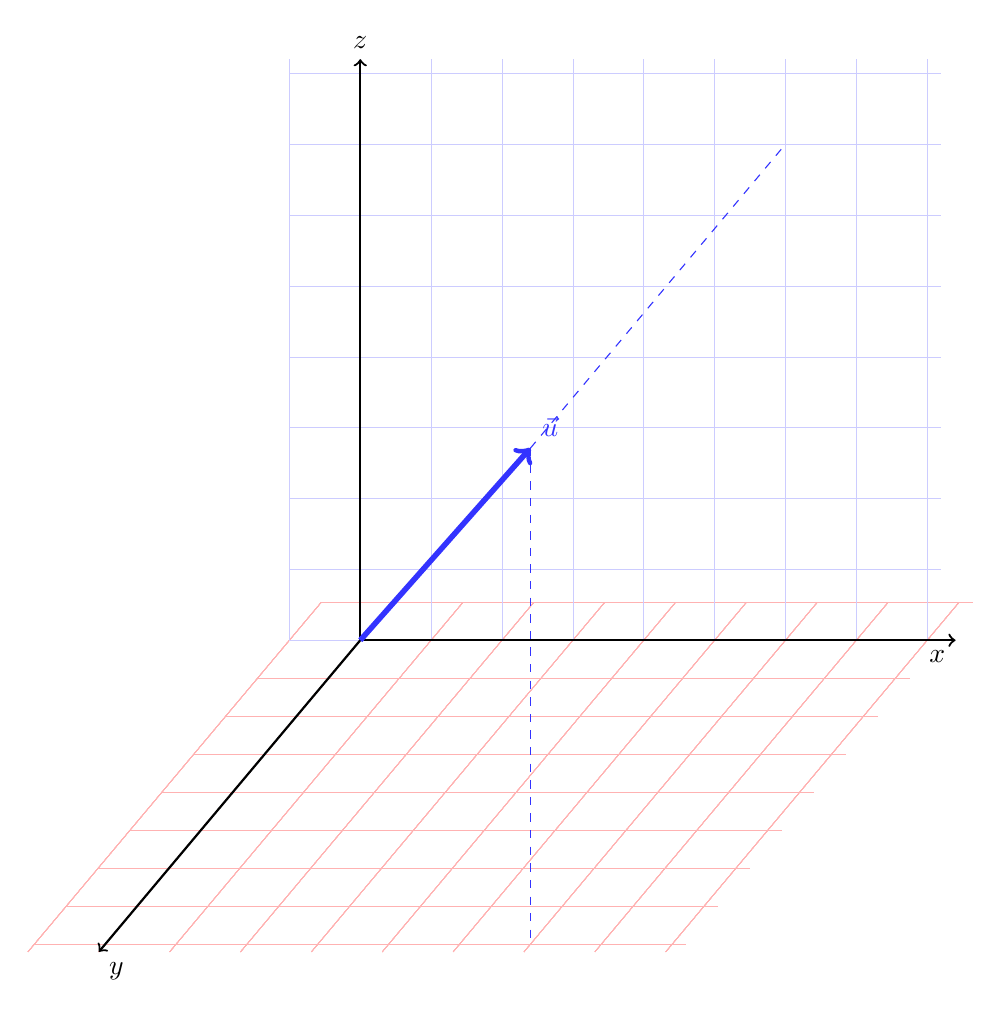
\begin{tikzpicture}[scale=1.8]
%standard tikz coordinate definition using x, y, z coords
    \coordinate (O) at (0,0,0);

\tikzset{
    x={(0:1cm)},y={(230:0.7cm)},z={(90:1cm)}
  }
 %draw a grid in the x-y plane
    \foreach \x in {-0.5,0,...,4}
        \foreach \y in {-0.5,0,...,4}
        {
            %eje xy
            \draw[very thin,red!30] (\x,-0.5) -- (\x,4.1);
            \draw[very thin,red!30] (-0.5,\y) -- (4.1,\y);
        }
%tikz-3dp %draw a grid in the x-z plane
    \foreach \x in {-0.5,0,...,4}
        \foreach \y in {0,0.5,...,4}
        {
            %eje xz
            \draw[very thin,blue!20] (\x,0,0) -- (\x,0,4.1);
            \draw[very thin,blue!20] (-0.5,0,\y) -- (4.1,0,\y);
        }
%draw axes
    \draw[->,thick] (0,0,0) -- (4.2,0,0) node[anchor=north east]{$x$};
    \draw[->,thick] (0,0,0) -- (0,4.1,0) node[anchor=north west]{$y$};
    \draw[->,thick] (0,0,0) -- (0,0,4.1) node[anchor=south]{$z$};

%draw a vector from O to P
    \draw[line width=2pt,blue!80,->] (O) -- (3,4,3.5)node[anchor=south west]{$\boldsymbol{\vec{u}}$};
    \draw[blue!80,dashed] (3,4,3.5)--(3,0,3.5);
    \draw[blue!80,dashed] (3,4,3.5)--(3,4,0);
\end{tikzpicture}




    Adicionalmente, los vectores poseen una \textbf{dimension}, esta representa
    la cantidad de coordenadas las cuales cubre. Los vectores mas usados son
    los bidimensionales, que poseen 2 coordenadas, $X,Y$ y representan el plano
    o espacio bidimensiona, son duplas ordenadas y pertenecen al espacio
    $\mathbb{R}^2$ y los tridimensionales, que utilizan 3 coordenadas $X,Y,Z$ y
    representan el espacio tridimensional perteneciendo al espacio
    $\mathbb{R}^3$.

    De igual forma, pueden utilizarse tantas dimensiones como hagan falta y el
    vector pertenecera al espacio $\mathbb{R}^n$ donde $n$ es la cantidad de
    coordenadas que posee y es un numero natural.

    Cabe destacar que estos vectores tambien son muy utilizados ya que permiten
    extrapolar fenomenos fisicos de mas variables, como por ejemplo el
    comportamiento de una caldera, o en el caso de 4 dimensiones cubrir tambien
    el tiempo $(x,y,z,t)$ y describir una fuerza o suceso en un espacio y
    tiempo determinado.

    Los vectores normalmente se utilizan para representar fuerzas, movimientos,
    variaciones, es decir cualquier condicion fisica que implica una potencia o
    cambio ejercido en una direccion particular.

    Por simplificacion, se trabajara en su mayotia con vectores en
    $\mathbb{R}^2$ y en $\mathbb{R}^3$ mas todos los conceptos son
    Extrapolables.

    Las operaciones, basicas, que se realizan con vectores son la suma
    algebraica, multiplicacion por un escalar. Adicionalmente esta definida la
    multiplicacion entre vectores como \textbf{producto punto} y
    \textbf{producto cruz}.

    \textbf{la division vectorial no esta definida!}, sin embargo, para ciertos
    tipos de vectores como fasores o numeros complejos se define una
    multiplicacion y una division especial.



    \subsubsection{Representacion}

    Los vectores pueden ser representados de 2 formas, mediante la descripcion
    individual de sus caracteristicas o mediante una magnitud y uno angulos de
    referencia. Ambas formas de representacion son equivalentes y se pueden
    llevar de una forma a otra.

    La forma de magnitud y angulo suele ser utilizada para vectores en
    $\mathbb{R}^2$ y mas especificamente en un conjunto de vectores con propiedades
    adicionales como lo son los numeros complejos, ya que es facil la
    transformacion, el producto y la division definido \textbf{unicamente para
    ellos} y para representarlos solamente se necesita un
    angulo. Para vectores de mayor dimension suele usarse la representacion por
    coordenadas, esto es debido a que para representar una linea en 3
    direcciones hacen falta al menos 2 angulos, uno de giro horizontal y otro
    vertical (a esto se le conoce como coordenadas esfericas).


    \subsubsection{Representacion en coordenadas rectangulares}

    Esta forma de representacion se basa en descomponer el vector en los
    valores asociados que poseen en cada eje. Por ejemplo, si el vector es de
    $\mathbb{R}^2$ tiene coordenadas $x$ e $y$, por lo tanto el vector puede
    ser representado como la union del origen (o un punto de referencia
    cualquiera) y los desplazamientos correspondientes en los ejes X,Y , si el
    vector es de 3 coordenadas, entonces serian X,Y,Z y asi sucesivamente. A
    este tipo de coordenadas se le conocen como \textbf{ coordenadas
    cartesianas o rectangulares}.

    De esta forma, un vector puede escribirse de 2 formas, como tupla ordenada
    o como suma de componentes, en donde cada componente va a estar indicada
    por un \textbf{vector unitario}, el cual no es mas que una letra la cual
    indica a que eje corresponde; $\hat{\imath}$ para x, $\hat{\jmath}$ para y,
    $\hat{k}$ para k.

    De esta forma, un vector puede ser escrito de la forma:

    $$\vec{v}=(v_1,v_2,v_3,\cdots,v_n),\ v_i \in \mathbb{R}$$


    o de la forma:

    $$\vec{v}=v_1\cdot\hat{\imath}+v_2\cdot\hat{\jmath}+v_3\cdot\hat{k}+\cdots$$

    Graficamente, estas composiciones son:

    Para 2 dimensiones:


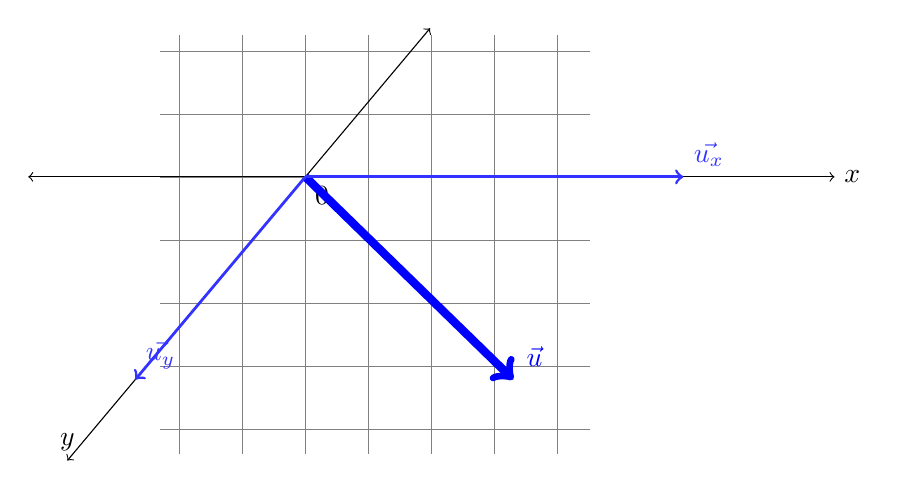
\begin{tikzpicture}[scale=1.6]
    \draw[style=help lines,step=0.5cm] (-2.1,-2.1)grid(4.1,4.1);
    \draw[<->] (-2.2,0)--(4.2,0) node[right]{$x$};
    \draw[<->] (0,-2.2)--(0,4.2) node[above]{$y$};
    \draw (0,0) node[anchor=north west ]{0};

    \draw[line width=3pt,blue,->](0,0)--(3,3) node[anchor=south west]{$\boldsymbol{\vec{u}}$};


    \draw[line width=1pt,blue!80,->](0,0)--(3,0) node[anchor=south west]{$\boldsymbol{\vec{u_x}}$};
    \draw[line width=1pt,blue!80,->](0,0)--(0,3) node[anchor=south west]{$\boldsymbol{\vec{u_y}}$};

\end{tikzpicture}

    Para 3 dimensiones:


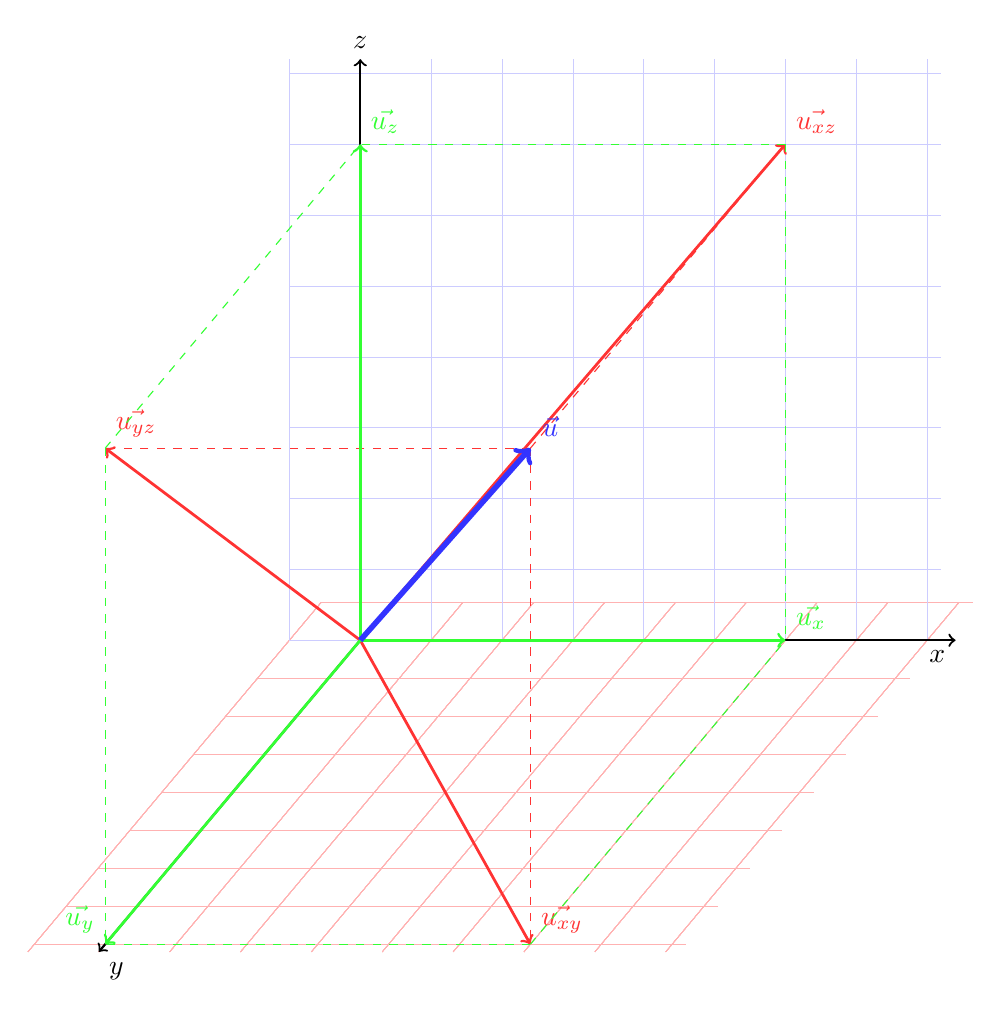
\begin{tikzpicture}[scale=1.8]
%standard tikz coordinate definition using x, y, z coords
    \coordinate (O) at (0,0,0);

\tikzset{
    x={(0:1cm)},y={(230:0.7cm)},z={(90:1cm)}
  }
 %draw a grid in the x-y plane
    \foreach \x in {-0.5,0,...,4}
        \foreach \y in {-0.5,0,...,4}
        {
            %eje xy
            \draw[very thin,red!30] (\x,-0.5) -- (\x,4.1);
            \draw[very thin,red!30] (-0.5,\y) -- (4.1,\y);
        }
%tikz-3dp %draw a grid in the x-z plane
    \foreach \x in {-0.5,0,...,4}
        \foreach \y in {0,0.5,...,4}
        {
            %eje xz
            \draw[very thin,blue!20] (\x,0,0) -- (\x,0,4.1);
            \draw[very thin,blue!20] (-0.5,0,\y) -- (4.1,0,\y);
        }
%draw axes
    \draw[->,thick] (0,0,0) -- (4.2,0,0) node[anchor=north east]{$x$};
    \draw[->,thick] (0,0,0) -- (0,4.1,0) node[anchor=north west]{$y$};
    \draw[->,thick] (0,0,0) -- (0,0,4.1) node[anchor=south]{$z$};

%draw a vector from O to P

    \draw[line width=1pt,red!80,->] (O) -- (0,4,3.5)node[anchor=south west]{$\boldsymbol{\vec{u_{yz}}}$} ;
    \draw[line width=1pt,red!80,->] (O) -- (3,0,3.5)node[anchor=south west]{$\boldsymbol{\vec{u_{xz}}}$} ;
    \draw[line width=1pt,red!80,->] (O) -- (3,4,0)node[anchor=south west]{$\boldsymbol{\vec{u_{xy}}}$} ;

    \draw[red!80,dashed] (3,4,3.5)--(3,0,3.5);
    \draw[red!80,dashed] (3,4,3.5)--(3,4,0);
    \draw[red!80,dashed] (3,4,3.5)--(0,4,3.5);

    \draw[line width=1pt,green!80,->] (O) -- (3,0,0)node[anchor=south west]{$\boldsymbol{\vec{u_{x}}}$} ;
    \draw[line width=1pt,green!80,->] (O) -- (0,4,0)node[anchor=south east]{$\boldsymbol{\vec{u_{y}}}$} ;
    \draw[line width=1pt,green!80,->] (O) -- (0,0,3.5)node[anchor=south west]{$\boldsymbol{\vec{u_{z}}}$} ;


    \draw[green!80,dashed] (3,0,3.5)--(0,0,3.5);
    \draw[green!80,dashed] (3,0,3.5)--(3,0,0);

    \draw[green!80,dashed] (0,4,3.5)--(0,4,0);
    \draw[green!80,dashed] (0,4,3.5)--(0,0,3.5);

    \draw[green!80,dashed] (3,4,0)--(3,0,0);
    \draw[green!80,dashed] (3,4,0)--(0,4,0);

    \draw[line width=2pt,blue!80,->] (O) -- (3,4,3.5)node[anchor=south west]{$\boldsymbol{\vec{u}}$} ;
\end{tikzpicture}




    Ejemplos:

    $$\vec{V}=(2,1)=2\hat{\imath}+1\hat{\jmath}$$
    $$\vec{V}=(-3,8)=-3\hat{\imath}+8\hat{\jmath}$$
    $$\vec{V}=(-21,-35)=-21\hat{\imath}-35\hat{\jmath}$$

    $$\vec{V}=(3,4,7)=3\hat{\imath}+4\hat{\jmath}+7\hat{k}$$
    $$\vec{V}=(-2,13,9)=-2\hat{\imath}+13\hat{\jmath}+9\hat{k}$$
    $$\vec{V}=(32,-4,-22)=32\hat{\imath}-4\hat{\jmath}-22\hat{k}$$


    \subsubsection{Representacion en magnitud y angulos}

    La otra forma de representar un vector es mediante una magnitud (que
    representa el tamaño del segmento-recta) y uno o mas angulos, los cuales
    son tomados con respecto a un punto de referencia y permiten orientar el
    vector en el espacio. Este tipo de coordenadas es conocido como
    \textbf{coordenadas polares} para 2 variables-ejes y \textbf{coordenadas
    esfericas} para 3 variables-ejes. Se escribe de la forma:

    $$\vec{V}= magnitud \phase{\theta} $$
    $$\vec{V}= magnitud  \phase{\theta}\phase{\phi} $$

    Donde, $magnitud$ se suele representar con la letra $r$ y los angulos
    suelen venir expresados en grados, ademas, $\theta$ mide el plano XY y
    $\phi$ el angulo con el eje Z. Y estan limitados por:


     \begin{align*}
         0\leq r&<\infty & 0\leq\theta&<2\pi & 0\leq\phi&\leq\pi \\
         0\leq r&<\infty & 0^\circ\leq\theta&<360^\circ & 0^\circ\leq\phi&\leq180^\circ
    \end{align*}

    Cabe resaltar que la nomenclatura puede variar y en algunos textos $\theta$
    se cambia por $\phi$, esto es debido a una falta de estadarizacion (como los
    cm y pulgadas, kg y libras, etc) en este texto se utilizara la convencion
    antes descrita para evitar confusiones, ya que en polares se usa $\theta$ para
    el plano XY.

    Ejemplos:


    $$\vec{V}=12 \phase{38^\circ} $$
    $$\vec{V}=23,22 \phase{98^\circ} $$
    $$\vec{V}=87,9 \phase{128^\circ} $$

    $$\vec{V}=45 \phase{12^\circ}\phase{30^\circ} $$
    $$\vec{V}=5 \phase{342^\circ}\phase{120^\circ} $$
    $$\vec{V}=23 \phase{2^\circ}\phase{180^\circ} $$

    Ambas representaciones son equivalentes,y esta equivalencia se logra
    mediante la trigonometria, mas especificamente un triangulo rectangulo.



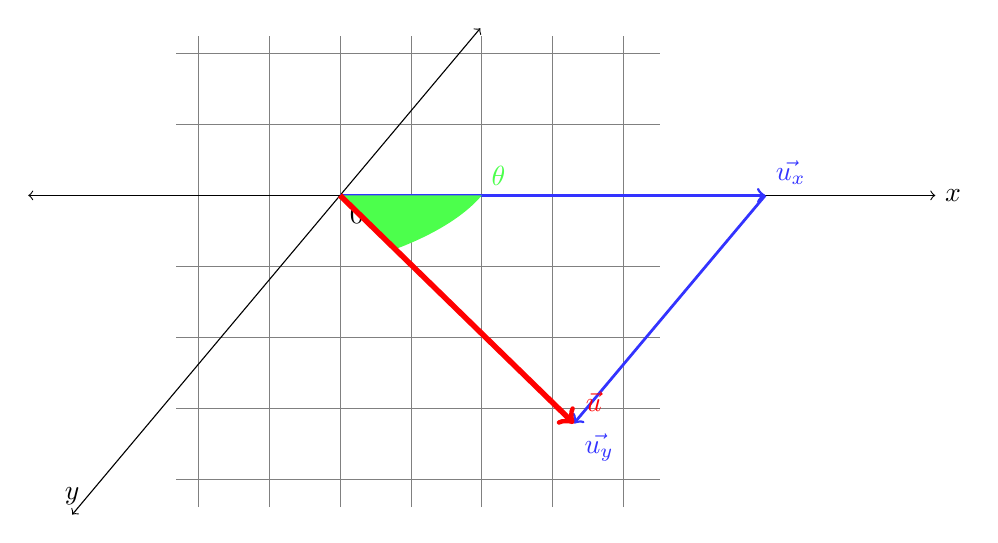
\begin{tikzpicture}[scale=1.8]
    \draw[style=help lines,step=0.5cm] (-2.1,-2.1)grid(4.1,4.1);
    \draw[<->] (-2.2,0)--(4.2,0) node[right]{$x$};
    \draw[<->] (0,-2.2)--(0,4.2) node[above]{$y$};
    \draw (0,0) node[anchor=north west ]{0};


    \draw[line width=1pt,blue!80,->](0,0)--(3,0) node[anchor= south west]{$\boldsymbol{\vec{u_x}}$};
    \draw[line width=1pt,blue!80,->](3,0)--(3,3) node[anchor=north  west]{$\boldsymbol{\vec{u_y}}$};
    \fill[green!70] (0,0)--(1,0) node[anchor=south west]{$\theta$} -- (1,0)  arc [start angle=0,end angle=45,x radius=1, y radius=1] ;

    \draw[line width=2pt,red,->](0,0)--(3,3) node[anchor=south west]{$\boldsymbol{\vec{u}}$};
\end{tikzpicture}


\tdplotsetmaincoords{60}{110}
\begin{tikzpicture}[scale=1.8,tdplot_main_coords]
%standard tikz coordinate definition using x, y, z coords
    \coordinate (O) at (0,0,0);

\tikzset{
    x={(0:1cm)},y={(230:0.7cm)},z={(90:1cm)}
  }
 %draw a grid in the x-y plane
    \foreach \x in {-0.5,0,...,4}
        \foreach \y in {-0.5,0,...,4}
        {
            %eje xy
            \draw[very thin,red!30] (\x,-0.5) -- (\x,4.1);
            \draw[very thin,red!30] (-0.5,\y) -- (4.1,\y);
        }
%tikz-3dp %draw a grid in the x-z plane
    \foreach \x in {-0.5,0,...,4}
        \foreach \y in {0,0.5,...,4}
        {
            %eje xz
            \draw[very thin,blue!20] (\x,0,0) -- (\x,0,4.1);
            \draw[very thin,blue!20] (-0.5,0,\y) -- (4.1,0,\y);
        }
%draw axes
    \draw[->,thick] (0,0,0) -- (4.2,0,0) node[anchor=north east]{$x$};
    \draw[->,thick] (0,0,0) -- (0,4.1,0) node[anchor=north west]{$y$};
    \draw[->,thick] (0,0,0) -- (0,0,4.1) node[anchor=south]{$z$};

%draw a vector from O to P

    \draw[red!80,dashed] (3,4,3.5)--(3,4,0);

    \begin{scope}[canvas is xy plane at z=0, thick]
        \draw (1,0) arc (0:53.13:1) ;
        \draw (1,0) node[anchor=north west ]{$\theta$};
    \end{scope}

    \tdplotsetthetaplanecoords{53.13}
    \tdplotdrawarc[tdplot_rotated_coords]{(0,0,0)}{1}{0}{40.5729}{anchor=south west}{$\phi$}

    \draw[line width=1pt,red!80,->] (O) -- (3,4,0)node[anchor=south west]{$\boldsymbol{\vec{u_{xy}}}$} ;
    \draw[line width=2pt,blue!80,->] (O) -- (3,4,3.5)node[anchor=south west]{$\boldsymbol{\vec{u}}$} ;
\end{tikzpicture}


    Como se observa en la imagen, y se sabe de la representacion por
    coordenadas, un vector puede representarse como sus coordenadas en los
    ejes, estas representaciones forman los catetos del triangulo y la magnitud
    total representa la hipotenusa del mismo. De esta forma, se tiene que:

    Para 2 variables:

    polares a cartesianas
    $$\vec{V_x}= r\cdot cos(\theta)$$
    $$\vec{V_y} =  r\cdot sen(\theta)$$

    cartesianas a polares
    $$ r = \sqrt{V_x ^2+v_y^2}$$
    $$\theta= arctan\left(\frac{V_y}{V_x}\right)$$



    para3 variables:

    esfericas a cartesianas
    $$\vec{V_x}= r\cdot cos(\theta) \cdot sin(\phi)$$
    $$\vec{V_y} = r\cdot sen(\theta)\cdot sin(\phi)$$
    $$\vec{V_z}=r\cdot cos(\phi)$$

    cartesianas a esfericas
    $$ r = \sqrt{V_x ^2+v_y^2+v_z^2}$$
    $$\theta= arctan\left(\frac{V_y}{V_x}\right)$$
    $$\phi = arcos\left(\frac{V_z}{r}\right)$$


    Ejemplos:


    Transformar a polares:

     \begin{align*}
         \vec{V}&=(2,1) \\
         r &= \sqrt{2^2+1^2}  \rightarrow r= \sqrt{5} \\
         \theta&= arctan\left(\frac{1}{2}\right)  \rightarrow \theta= 26,57 ^\circ \\
    \end{align*}

     \begin{align*}
         \vec{V}&=(-3,8) \\
         r &= \sqrt{(-3)^2+8^2} \rightarrow r= \sqrt{73} \\
         \theta&= arctan\left(\frac{8}{-3}\right)  \rightarrow \theta= -69,44^\circ =-69,44^\circ+360^\circ=290.56 \\
    \end{align*}

     \begin{align*}
         \vec{V}&=(-21,-35) \\
         r &= \sqrt{(-21)^2+(-35)^2}  \rightarrow r= 7\sqrt{34} \\
         \theta&= arctan\left(\frac{-35}{-21}\right)  \rightarrow \theta= 59,04^\circ\\
    \end{align*}

    Transformar a esfericas:

    \begin{align*}
        \vec{V}&=(3,4,7) \\
        r &= \sqrt{3^2+4^2+7^2} \rightarrow w =\sqrt{74}  \\
        \theta&= arctan\left(\frac{4}{3}\right)  \rightarrow \theta= 53,13^\circ \\
        \phi &=arcos\left(\frac{7}{\sqrt{74}}\right)  \rightarrow \phi= 35,54^\circ\\
    \end{align*}

    \begin{align*}
        \vec{V}&=(-2,13,9) \\
        r &= \sqrt{(-2)^2+13^2+9^2}  \rightarrow w =\sqrt{254}  \\
        \theta&= arctan\left(\frac{13}{-2}\right)  \rightarrow \theta= -81,25^\circ= 278.75^\circ\\
        \phi &= arcos\left(\frac{9}{\sqrt{254}}\right)  \rightarrow \phi=  55,62^\circ\\
    \end{align*}

    \begin{align*}
        \vec{V}&=(32,-4,-22) \\
        r &= \sqrt{32^2+(-4)^2+22^2}  \rightarrow w =2\sqrt{381}  \\
        \theta&= arctan\left(\frac{13}{-2}\right)  \rightarrow \theta= -7,13^\circ=352,87^\circ \\
        \phi &= arcos\left(\frac{-22}{2\sqrt{381}}\right)  \rightarrow \phi= 124,3^\circ\\
    \end{align*}

    Transformar a rectangulares
    \begin{align*}
        \vec{V}&=12\phase{38^\circ}  \\
        \vec{V_x}&= 12\cdot cos(38^\circ) \rightarrow \vec{V_x} = \sqrt{9,456} \\
        \vec{V_y}& =  12\cdot sen(38^\circ)  \rightarrow \vec{V_y}= \sqrt{7,388} \\
    \end{align*}

    \begin{align*}
        \vec{V}&=23,22 \phase{98^\circ}  \\
        \vec{V_x}&= 23,22\cdot cos(98^\circ)  \rightarrow \vec{V_x} = \sqrt{18,298} \\
        \vec{V_y}& =  23,22\cdot sen(98^\circ)  \rightarrow \vec{V_y}= \sqrt{14.296} \\
    \end{align*}

    \begin{align*}
        \vec{V}&=87,9 \phase{128^\circ}  \\
        \vec{V_x}&= 87,9\cdot cos(128^\circ) \rightarrow \vec{V_x} = \sqrt{-54,117} \\
        \vec{V_y}& =  87,9\cdot sen(128^\circ)  \rightarrow \vec{V_y}= \sqrt{69.266} \\
    \end{align*}


    \begin{align*}
        \vec{V}&=45 \phase{12^\circ}\phase{30^\circ} \\
        \vec{V_x}&= 45\cdot cos(12^\circ) \cdot sin(30^\circ)  \rightarrow \vec{V_x} = \sqrt{22,008} \\
        \vec{V_y} &= 45\cdot sen(12^\circ)\cdot sin(30^\circ) \rightarrow \vec{V_x} = \sqrt{4,678} \\
        \vec{V_z}&=45\cdot cos(30^\circ)  \rightarrow \vec{V_x}= \sqrt{38,971} \\
    \end{align*}

    \begin{align*}
        \vec{V}&=5 \phase{342^\circ}\phase{120^\circ}\\
        \vec{V_x}&= 5\cdot cos(342^\circ) \cdot sin(120^\circ)   \rightarrow \vec{V_x} = \sqrt{4,118} \\
        \vec{V_y} &=5r\cdot sen(342^\circ)\cdot sin(120^\circ)  \rightarrow \vec{V_x} = \sqrt{-1,338} \\
        \vec{V_z}&=5\cdot cos(120^\circ)  \rightarrow \vec{V_x} = \sqrt{-2,5} \\
    \end{align*}

    \begin{align*}
        \vec{V}&=23 \phase{0^\circ}\phase{180^\circ}\\
        \vec{V_x}&= 23\cdot cos(2^\circ) \cdot sin(180^\circ)   \rightarrow \vec{V_x} = \sqrt{0} \\
        \vec{V_y} &= 23\cdot sen(2^\circ)\cdot sin(180^\circ)  \rightarrow \vec{V_x} = \sqrt{0} \\
        \vec{V_z}&= 23\cdot cos(180^\circ)  \rightarrow \vec{V_x} = \sqrt{-23} \\
    \end{align*}


    \subsubsection{Suma}

    La suma de vectores se realiza con los vectores en su forma cartesiana, es
    decir,\textbf{ para poder sumar 2 vectores debemos llevarlo a su forma
    rectangular}, La forma en la que se hace la suma es simplemente sumar sus
    componentes internas, es decir su representacion en $x$ con su respectivo
    par, la de $y$ con $y$ y asi sucesivamente.

    Sean $\vec{v},\vec{u}$ dos vectores cualesquiera de $\mathbb{R}^n$ tal que:

    $$\vec{v}=(v_1,v_2,v_3,\cdots,v_n)\ ; \vec{u}=(u_1,u_2,u_3,\cdots,u_n)$$
    $$\vec{r}=\vec{v+u}=(v_1+u_1,v_2+u_2,v_3+u_3,\cdots,v_n+u_n)$$

    \textbf{Recuerde que,} una suma algebraica es la suma con signo de los
    elementos, esto quiere decir que incluye a la resta ya que si se suman
    numeros de signos opuestos es lo mismo a restarlos.

    Graficamente, la forma mas sencilla es dibujar el primer vector en el
    origen y en su extremo dibujar el siguiente vector (el que se le sumara
    algebraicamente), luego se unen el origen del primer vector (corresponde
    con el origen del plano por como se definió) y el fin del segundo vector
    y este es el vector suma resultante.

    Graficamente, para $\mathbb{R}^2$:


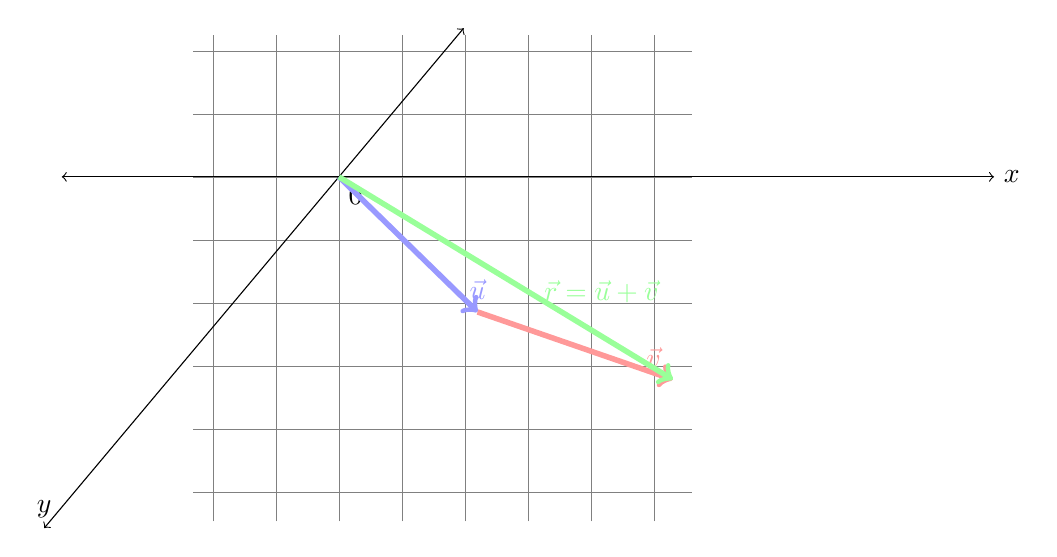
\begin{tikzpicture}[scale=1.6]
    \draw[style=help lines,step=0.5cm] (-2.1,-2.1)grid(5.1,5.1);
    \draw[<->] (-2.2,0)--(5.2,0) node[right]{$x$};
    \draw[<->] (0,-2.2)--(0,5.2) node[above]{$y$};
    \draw (0,0) node[anchor=north west ]{0};

    \draw[line width=2pt,blue!40,->](0,0)--(2,2) node[anchor=south]{$\boldsymbol{\vec{u}}$};

    \draw[line width=2pt,red!40,->](2,2)--(4,3) node[anchor=south east ]{$\boldsymbol{\vec{v}}$};

    \draw[line width=2pt,green!40,->](0,0)--(4,3) ;
    \draw[line width=2pt,green!40] (2.3,1.7) node[anchor=west ]{$\boldsymbol{\vec{r}=\vec{u}+\vec{v}}$};
\end{tikzpicture}

    Ejemplos: Sumar los siguientes vectores

    \begin{align*}
        \vec{V}& =(2,1) \ \ ;\ \ \ \vec{U} =(-3,8)		\\
        \vec{R}&= (2-3 ,1+8 )   \rightarrow \vec{R} = (-1 ,9  )
    \end{align*}

    \begin{align*}
        \vec{V}& =(-21,-35)  \ \ ;\ \ \  \vec{U} =(-3,8)		\\
        \vec{R}&= (-21-3 ,-35+8  )  \rightarrow \vec{R} = (-24 ,-27  )
    \end{align*}

    \begin{align*}
        \vec{V}& =(-21,-35)  \ \ ;\ \ \  \vec{U} =(2,1)		\\
        \vec{R}&= (-21+2 , -35+1 )   \rightarrow \vec{R} = (-19 ,-34  )
    \end{align*}




    \begin{align*}
        \vec{V}& =(3,4,7)  \ \ ;\ \ \   \vec{U} =(-2,13,9)		\\
        \vec{R}&= (3-2 ,4+13 ,7+9 )   \rightarrow \vec{R} = (4,17,16 )
    \end{align*}

    \begin{align*}
        \vec{V}& =(3,4,7)  \ \ ;\ \ \  \vec{U} =(32,-4,-22)		\\
        \vec{R}&= (3+32, 4-4,7-22 )  & \rightarrow \vec{R} &= ( 35,0 ,-15 )
    \end{align*}

    \begin{align*}
        \vec{V}& =(-2,13,9)  \ \ ;\ \ \   \vec{U} =(32,-4,-22)		\\
        \vec{R}&= (-2+32 ,13-4 ,9-22 )  \rightarrow \vec{R} = (30, 9,-13 )
    \end{align*}


    \subsubsection{Producto por escalar}

    El producto por escalar es una operacion que toma un vector cualesquiera
    $\vec{v} \in \mathbb{R}^n$ y un escalar (numero) cualquiera $\alpha \in
    \mathbb{R}$. Consiste en multiplicar ese escalar por todos los elementos del
    vector modificando de esta forma su magnitud. Cuando el vector se encuentra
    en coordenadas polares o esfericas solamente se modifica la magnitud,
    multiplicandola por el escalar, el angulo permanece igual.

    Sean $\vec{v}$ un  vector cualesquiera de $\mathbb{R}^n$  tal que:

    $$\vec{v}=(v_1,v_2,v_3,\cdots,v_n)\ ; \alpha \in \mathbb{R} $$
    $$\vec{r}=\alpha\cdot\vec{v}=(v_1\cdot\alpha,v_2\cdot\alpha,v_3\cdot\alpha,\cdots,v_n\cdot\alpha)$$

    Graficamente:
    \begin{itemize}
        \item Aumenta su tamaño si $|\alpha| >1$.
        \item Reduce su tamaño si $|\alpha| <1$.

        \item Invierte su direccion y  sigue las reglas de la magnitud anteriores
            si $\alpha<0$.

        \item Permanece igual si $\alpha=1$.
        \item Se anula se $\alpha = 0$.
    \end{itemize}


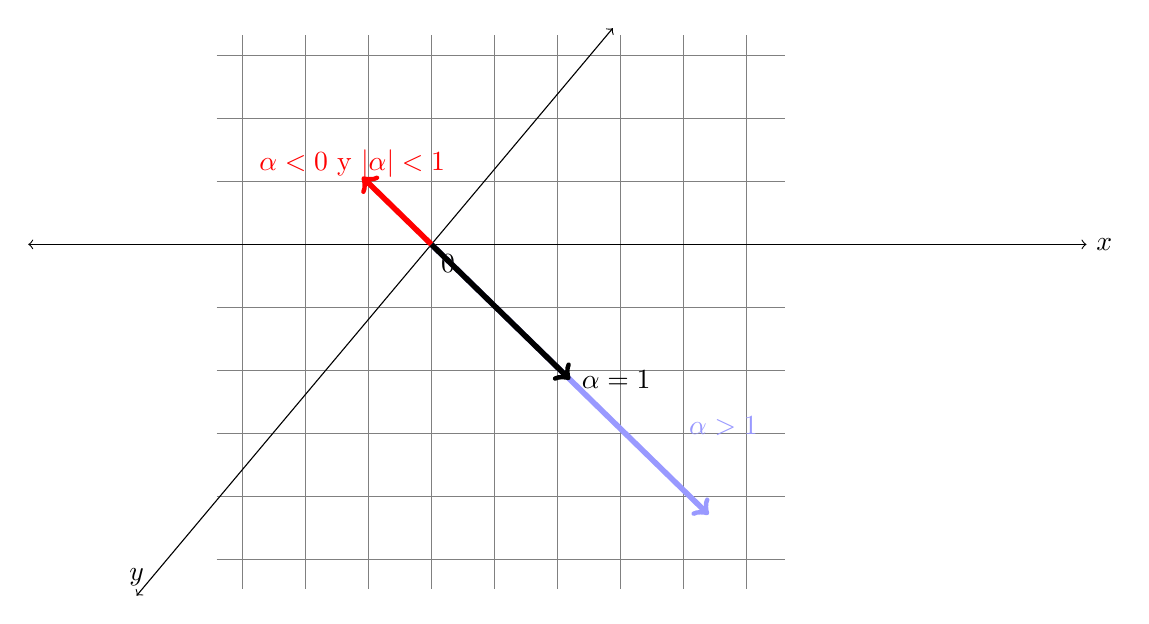
\begin{tikzpicture}[scale=1.6]
    \draw[style=help lines,step=0.5cm] (-3.1,-3.1)grid(5.1,5.1);
    \draw[<->] (-3.2,0)--(5.2,0) node[right]{$x$};
    \draw[<->] (0,-3.2)--(0,5.2) node[above]{$y$};
    \draw (0,0) node[anchor=north west ]{0};

    \draw[line width=2pt,blue!40,->](0,0)--(4,4) ;
    \draw[line width=2pt,blue!40] (3.3,3) node[anchor=south west]{$\alpha>1$};

    \draw[line width=2pt,red,->](0,0)--(-1,-1) ;
    \draw[line width=2pt,red] (-2,-1.2) node[anchor=west ]{$\alpha<0$ y $|\alpha|<1$};

    \draw[line width=2pt,->](0,0)--(2,2) node[anchor=west]{$\alpha=1$};
\end{tikzpicture}


    Ejemplos, multiplicar los siguientes vectores por los escalares:

    \begin{align*}
        \vec{V}& =(2,1)  \ \ ;\ \ \  \alpha =3 		\\
        \vec{R}&= (2\times3,1\times3 )   \rightarrow \vec{R}= (6,3 )
    \end{align*}

    \begin{align*}
        \vec{V}& =(-3,8)  \ \ ;\ \ \  \alpha = 8		\\
        \vec{R}&= (-3 \times8,8 \times8 )   \rightarrow \vec{R}= (-24,64 )
    \end{align*}

    \begin{align*}
        \vec{V}& =(-21,-35)  \ \ ;\ \ \ \alpha = -5		\\
        \vec{R}&= (-21 \times-5,-35 \times-5)  \rightarrow \vec{R} = (105,175 )
    \end{align*}





    \begin{align*}
        \vec{V}& =(3,4,7)  \ \ ;\ \ \  \alpha= -9	\\
        \vec{R}&= (3 \times-9,4 \times-9,7 \times-9  )  \rightarrow \vec{R}= (-27,-36,-63 )
    \end{align*}

    \begin{align*}
        \vec{V}& =(-2,13,9)  \ \ ;\ \ \  \alpha = 12 		\\
        \vec{R}&= (-2 \times12, 13 \times12, 9 \times12)  \rightarrow \vec{R}= (-24,156,108)
    \end{align*}

    \begin{align*}
        \vec{V}& =(32,-4,-22)  \ \ ;\ \ \  \alpha = -1		\\
        \vec{R}&= (32 \times-1, -4 \times-1, -22 \times-1 )  \rightarrow \vec{R}= (-32,4,22)
    \end{align*}




    \subsubsection{Multiplicacion entre vectores}

    La multiplicacion entre vectores es una propiedad definida de una forma
    muy distinta a la multiplicacion numerica. Esto se debe a la complejidad de
    los vectores la cual permite defini varios tipos de multiplicaciones posibles
    las cuales tienen sentido. Las 2 Multiplicacionesmas conocidas son \textbf{
    el producto punto y el producto cruz}, ademas de esto existen otras formas
    de realizar multiplicaciones como la es la de los numeros complejos, siendo
    esta definida de tal forma que permite incluso crear una division.

    Los producto punto y producto cruz \textbf{No tienen operacion inversa} y es
    por esto que \textbf{no existe la division vectorial}.

    \subsubsection{Producto punto}

    Este tipo de multiplicacion es realizable par todos los vectores y da como
    resultado un escalar, es decir un numero.

    Se escribe de la forma: $\vec{r} = \vec{v}\cdot\vec{u}$, con
    $\vec{v},\vec{u}$ vectores cualesquiera.

    La forma de definir este producto varia, existen varios procedimientos
    equivalentes, las dos mas conocidas son con la norma de cada uno de los vectores
    y el angulo entre vectores, y el que se trabajara aca que es una suma del
    producto entre los componentes del vector. Es decir:

    Sean $\vec{v},\vec{u}$ dos vectores cualesquiera de $\mathbb{R}^n$ tal que:

    \begin{align*}
        \vec{v}&=(v_1,v_2,v_3,\cdots,v_n) \ \ ;\ \ \ \vec{u}=(u_1,u_2,u_3,\cdots,u_n)\\
        \vec{r}&=\vec{v}\cdot\vec{u}= (v_1\cdot u_1,v_2 \cdot u_2,v_3 \cdot u_3,\cdots,v_n \cdot u_n)\rightarrow
        \vec{r}= \sum_{i=0}^{n} v_i\cdot u_i
    \end{align*}


    Ejemplos:

    \begin{align*}
        \vec{V}& =(2,1) \ \ ;\ \ \  \vec{U} =(-3,8)		\\
        \vec{R}&= 2\cdot-3 +1\dot8   \rightarrow \vec{R}= 2
    \end{align*}

    \begin{align*}
        \vec{V}& =(-21,-35)  \ \ ;\ \ \  \vec{U} &=(-3,8)		\\
        \vec{R}&= -21\cdot-3 +\ -35\cdot8    \rightarrow \vec{R}= -217
    \end{align*}

    \begin{align*}
        \vec{V}& =(-21,-35)  \ \ ;\ \ \ \vec{U} &=(2,1)		\\
        \vec{R}&= -21\cdot2 + -35\cdot1   \rightarrow \vec{R}= -77
    \end{align*}




    \begin{align*}
        \vec{V}& =(3,4,7)   \ \ ;\ \ \  \vec{U} =(-2,13,9)		\\
        \vec{R}&= 3\cdot-2 +4\cdot13 +7\cdot9   \rightarrow \vec{R} = 109
    \end{align*}

    \begin{align*}
        \vec{V}& =(3,4,7)  \ \ ;\ \ \  \vec{U} =(32,-4,-22)		\\
        \vec{R}&= 3\cdot32 + 4\cdot-4 +7\cdot22    \rightarrow \vec{R} = -74
    \end{align*}

    \begin{align*}
        \vec{V}& =(-2,13,9)  \ \ ;\ \ \   \vec{U} =(32,-4,-22)		\\
        \vec{R}&= -2\cdot32 + 13\cdot-4 +9\cdot-22 )  \rightarrow \vec{R} = -314
    \end{align*}

    \subsubsection{Producto cruz}

    Este tipo de multiplicacion da como resultado un vector, graficamente, da
    como resultado un vector perpendicular al plano ($90^\circ$) formado por
    los dos vectores
    que se multiplican, no es conmutativa ya que si se invierten los vectores
    se invierte la direccion del vector resultante y es utilizada mayormente en
    $\mathbb{R}^3$, en $\mathbb{R}^2$ esta division es un producto externo ya
    que la multiplicacion da como resultado un vector que no existe en este espacio
    (al ser perpendicular al plano X,Y se encuentra en el eje z el cual no esta
    definido en el plano cartesiano) y por esto no se realiza.

    Este producto vectorial es de mucha utilidad por su capacidad de entregar
    un vector perpendicular a los multiplicados y es una base fundamental para
    muchas aplicaciones de la ingenieria, arquitectura y fisica en general.

    Puede escribirse como calculo de determinantes, es lo que se utiliza en su
    mayoria para calculos de $\mathbb{R}^n$, pero para $\mathbb{R}^3$ se utiliza
    mucho mas una formula.

    Se escribe de la forma: $\vec{r} = \vec{u}\times\vec{v}$, con
    $\vec{u},\vec{v}$ vectores cualesquiera.

    y para $\mathbb{R}^3$ especificamente, con $\vec{u}=(u_x,u_y,u_z),
    \vec{v}=(v_x,v_y,v_z)$ esto es:

    $$\vec{r} = \vec{u}\times\vec{v} =
        (u_y\cdot v_z- u_z\cdot v_y)\hat{\imath}
        - (u_x\cdot v_z- u_z\cdot v_x)\hat{\jmath}
        +  (u_x\cdot v_y- u_y\cdot v_x)\hat{k}
    $$

    Esto significa que con $\vec{r} = (r_x,r_y,r_z)$, las componentes del vector
    son :

    \begin{align*}
        \vec{r_x}& = (u_y\cdot v_z- u_z\cdot v_y)\\
        \vec{r_y}&= -(u_x\cdot v_z- u_z\cdot v_x)\\
        \vec{r_z}&= (u_x\cdot v_y- u_y\cdot v_x)
    \end{align*}

    Ejemplos:

    \begin{align*}
        \vec{u}& =(3,4,7)   \ \ ;\ \ \  \vec{v} =(-2,13,9)		\\
        \vec{r_x}& = (4\cdot 9- 7\cdot 13) = -55 \\
        \vec{r_y}&= -(3\cdot 9- 7\cdot -2)= -41 \\
        \vec{r_z}&= (3\cdot 13- 4\cdot -2) = 47 \\
        \vec{r_z}&= \vec{u}\times\vec{v} = (-55,-41,47)
    \end{align*}

    \begin{align*}
        \vec{u}& =(3,4,7)  \ \ ;\ \ \  \vec{v} =(32,-4,-22)		\\
        \vec{r_x}& = (4\cdot -22 - 7\cdot -4)= -60\\
        \vec{r_y}&= -(3\cdot -22- 7\cdot 32) =290\\
        \vec{r_z}&= (3\cdot -4- 4\cdot 32) = -140\\
        \vec{r_z}&= \vec{u}\times\vec{v} = (-60,-290,-140)
    \end{align*}

    \begin{align*}
        \vec{u}& =(-2,13,9)  \ \ ;\ \ \   \vec{v} =(32,-4,-22)		\\
        \vec{r_x}& = (13\cdot -22- 9\cdot -4)= -250\\
        \vec{r_y}&= -(-2\cdot -22- 9\cdot 32)= 244\\
        \vec{r_z}&= (-2\cdot -4- 13\cdot 32) =-408\\
        \vec{r_z}&= \vec{u}\times\vec{v} = (-250, 244, -408)
    \end{align*}




\subsection{matrices}

una matriz es un arreglo bidimensional de números. Es decir, es una ampliacion de
los vectores con 2 dimensiones, usualmente a las operaciones que se pueden hacer
con las matrices se le conoce como algebra matricial. Cabe resaltar que tambien
existes arreglos de mas dimensiones llamados tensores que son tema de matematicas
muy avanzadas.

Hay 2 tipos de matrices, las cuadradas, conocidas como orden $n\times n$ las
cuales tienen el mismo numero de filas y columnas, $n$
y las rectangulares o mejor conocidas como de orden $n\times m$ donde $n$
representa la cantidad de filas y $m$ la cantidad de columnas. donde:
$ 1\leq  n < \infty$ y  $ 1\leq m < \infty$.
En el caso de que la matriz tenga 1 fila o 1 columna es un vector,

Una matriz se suele escribir por una letra mayuscula y sus componentes con la
misma letra minuscula y dos subindices, uno para las filas y otro para las
columnas tipicamente simbolizado por las letras $ij$($a_{filas\ columnas}=
a_{i\ j}$). Es decir, tienen la forma:

\begin{*equation}
    A =
    \begin{bmatrix}
        a_{1\ 1} & a_{1\ 2} & \cdots & a_{1\ m}\\
        a_{2\ 1} & a_{2\ 2} & \cdots & a_{2\ m}\\
        \vdots & \vdots & \ddots & \vdots\\
        a_{n\ 1} & a_{n\ 2} & \cdots & a_{n\ m}\\
    \end{bmatrix}
\end{*equation}


En las matrices se definen 3 operaciones basicas, estas son suma algebraica,
multiplicacion por un escalar y multiplicacion entre matrices. \textbf{La division
no esta definida}, ademas, existen muchas otras aplicaciones que se pueden
realizar con matrices como lo son la resolucion de sistemas de ecuaciones y
todo lo que esto implica.

\subsubsection*{Multiplicacion por escalar} \label{Multiplicacion_escalar}

Este tipo de operacion no tiene limitaciones en cuanto al tamaño de las matrices
y esta definida de igual forma que con los vectores, es decir, el escalar que
multiplica a la matriz multiplica a todos los elementos internos de la matriz.




\subsubsection*{Suma de matrices} \label{Sumadematrices}

Esta operacion esta limitada a las matrices de igual orden, es decir ambas
matrices deben de ser orden $n\times m$ para que la operacion pueda ser realizada
y esto es porque esta definida de forma que la suma de las matrices da como
resultado una nueva matriz del mismo tamaño ($n\times m) en donde cada elemento
es la suma de los elementos que estaban en la misma posicion que el resultante.
Igual que la suma de vectores.


\subsubsection*{Multiplicacion de matrices} \label{Multiplicaciondematrices}

Esta operacion no es conmutativa y esta sujeta a la condicion de que el
numero de columnas de la primera matriz debe ser igual al numero de filas de la
segunda matriz y da como resultado una matriz que tiene la cantidad de fiulas de
la primera matriz y la cantidad de columnas de la segunda matriz.











